\documentclass[11pt, aspectratio=169]{beamer}
%
% Choose how your presentation looks.
\usepackage{pgfpages}
\setbeameroption{hide notes}

\usepackage{helvet}
\usepackage{threeparttable}
\usepackage[default]{lato}
\usepackage{array}
\usepackage{tikz}
\usepackage{verbatim}
\usetikzlibrary{positioning}
\usetikzlibrary{calc}
\usetikzlibrary{arrows}
\usetikzlibrary{decorations.markings}
\usetikzlibrary{shapes.misc}
\usetikzlibrary{matrix,shapes,arrows,fit,tikzmark}
\usepackage{amssymb}
\usepackage{amsfonts}
\usepackage{amsmath}
\usepackage{mathpazo}
\usepackage{hyperref}
\usepackage{lipsum}
\usepackage{multimedia}
\usepackage{graphicx}
\usepackage{multirow}
\usepackage{graphicx}
\usepackage{dcolumn}
\usepackage{bbm}
\usepackage{changepage}
\usepackage{appendixnumberbeamer}

\definecolor{blue}{RGB}{0,114,178}
\definecolor{red}{RGB}{213,94,0}
\definecolor{yellow}{RGB}{240,228,66}
\definecolor{green}{RGB}{0,158,115}
\definecolor{gray}{RGB}{240,240,240}

\hypersetup{
  colorlinks={true},
  citecolor=green,
  linkbordercolor = {white},
  linkcolor = {blue}
}

\definecolor{MyBackground}{RGB}{255,253,218}

\newenvironment{transitionframe}{
  \setbeamercolor{background canvas}{bg=gray}
  \begin{frame}}{
    \end{frame}
}

\setbeamercolor{frametitle}{fg=blue}
\setbeamercolor{title}{fg=black}
\setbeamertemplate{footline}[frame number]
\setbeamertemplate{navigation symbols}{} 
\setbeamertemplate{itemize items}{-}
\setbeamercolor{itemize item}{fg=blue}
\setbeamercolor{itemize subitem}{fg=blue}
\setbeamercolor{enumerate item}{fg=blue}
\setbeamercolor{enumerate subitem}{fg=blue}
\setbeamercolor{button}{bg=MyBackground,fg=blue,}
\setbeamercolor{section in toc}{fg=blue}
\setbeamercolor{subsection in toc}{fg=red}
\setbeamersize{text margin left=1em,text margin right=1em} 

\newenvironment{wideitemize}{\itemize\addtolength{\itemsep}{10pt}}{\enditemize}

\mode<presentation>

% \AtBeginSection[]
% {
%   \begin{frame}
%        \frametitle{Contents}
%        \tableofcontents[currentsection]
%   \end{frame}
% }

% \AtBeginSubsection[]
% {
%   \begin{frame}
%        \frametitle{Contents}
%        \tableofcontents[currentsubsection]
%   \end{frame}
% }

\graphicspath{{Graphs/}}

\usepackage[english]{babel}
\usepackage[utf8]{inputenc}
\usepackage[T1]{fontenc}
\usepackage{makecell}
\usepackage{booktabs}
\usepackage[natbibapa]{apacite}

\def\bibfont{\scriptsize}

\title[Your Short Title]{\textcolor{blue}{Heterogeneity in the Returns to Education in Colombia}}
\author{Christian Posso \inst{1} \and Estefania Saravia \inst{2} \and Pablo Uribe \inst{3}}
\institute{\inst{1} Banco de la República \and \inst{2} UCLA \and \inst{3} World Bank}
\date{LACEA-LAMES 2023} %\today

\begin{document}

\tikzset{   
        every picture/.style={remember picture,baseline},
        every node/.style={anchor=base,align=center,outer sep=1.5pt},
        every path/.style={thick},
        }
\newcommand\marktopleft[1]{%
    \tikz[overlay,remember picture] 
        \node (marker-#1-a) at (-.3em,.3em) {};%
}
\newcommand\markbottomright[2]{%
    \tikz[overlay,remember picture] 
        \node (marker-#1-b) at (0em,0em) {};%
}
\tikzstyle{every picture}+=[remember picture] 
\tikzstyle{mybox} =[draw=black, very thick, rectangle, inner sep=10pt, inner ysep=20pt]
\tikzstyle{fancytitle} =[draw=black,fill=red, text=white]

\begin{frame}
  \maketitle
  \centering {\footnotesize The opinions and possible errors contained in this document are the sole responsibility of the authors and do not commit Banco de la Rep\'ublica or its Board of Directors.}
\end{frame}

\begin{frame}
    \frametitle{Contents}
    \tableofcontents
\end{frame}

%%%%%%%%%%%%%%%%% Introduction

\section{Introduction}

\begin{transitionframe}
  \begin{center}
    { \huge \textcolor{blue}{Introduction}}
  \end{center}
\end{transitionframe}

\begin{frame}{Motivation}
    \begin{wideitemize}
        \item There are, in general, significant returns to a college degree, although they are not constant across programs and may not benefit all students \citep{oreopoulos2013making}.
        \item Private returns to higher education have risen over time, and they are higher in low-income countries \citep{psacharopoulos2018returns}.
        \item Even if returns to education in Latin America are high, there is large heterogeneity based on a wide range of conditions \citep{ferreyra2017crossroads}.
        \begin{itemize}
            \item Human capital $\longrightarrow$ cognitive and non-cognitive abilities \citep{heckman2006effects}.
            \item Major \citep{altonji2021labor}.
            \item Initial conditions (e.g. city of origin).
        \end{itemize}
    \end{wideitemize}

\end{frame}

\begin{frame}{Pre-college scores, major and returns?}
    \begin{wideitemize}
        \item \citet{altonji2018costs} use SAT scores as a control with a sample from 15 Florida counties. Major returns are quite heterogeneous, especially when considering each major’s costs.
        \item \citet{ferreyra2022labor} use Saber 11 scores as a control. They are looking at the returns to short-cycle programs. They focus on 2005 high school graduates, and use GEIH and OLE for labor market outcomes.
        \item Returns often depend on the undergraduate major \citep{altonji2021labor}.
        \item Returns vary by major choice and type of major. There are distributional effects, and career trajectories as well as pre-collegiate measures of ability are important \citep{andrews2022returns}.
    \end{wideitemize}

\end{frame}

\begin{frame}{Preview}
    \begin{wideitemize}
        \item We use administrative data that link the pre-collegiate situation with higher education access and formal labor market outcomes for the entire population of \textbf{high school seniors in Colombia between 2001 and 2006}.
        \item One of few efforts in LA to have microdata on skills, higher education access and earnings for a whole country \citep{gomez2022returns,herrera2020economic,ferreyra2022labor}.
        \item Main takeaways:
        \begin{itemize}
            \item Skills matter.
            \item Experience matters.
            \item Geography matters a lot.
            \item Choice of major matters. 
        \end{itemize}
    \end{wideitemize}

\end{frame}

%%%%%%%%%%%%%%%%% Data

\section{Data}

\begin{transitionframe}
  \begin{center}
    { \huge \textcolor{blue}{Data}}
  \end{center}
\end{transitionframe}

\begin{frame}{Data}
    Three main sources:
    \vspace{0.2cm}
    \begin{wideitemize}
        \item \textbf{Saber 11} (2001-2006). We exclude 2005-1 due to high percentage of missing values in covariates.
        \item \textbf{SPADIES} (2001-2015). Keep people who started higher education at least in 2001. If a student shows up with several programs, keep the one he started first If it started both of them at the same time, keep the one with the earliest graduation date.
        \item \textbf{PILA} (2008-2019). At the semester level, keeping the last seen salary in a given semester and the month it was seen to include month FE.

    \end{wideitemize}

\end{frame}

\begin{frame}{Data}
    The data are merged in the following way:
    \vspace{0.2cm}
    \begin{enumerate}
        \item Use SPADIES ID to match to the Saber 11 ID. This links the pre-collegiate information to the higher education data.
        \item Randomly drop ID duplicates in order to match with the PILA panel.
        \item Match national ID numbers to anonymized ID’s (personabasicaid) from a ~20M crosswalk.
        \item After obtaining the personabasicaid, merge with PILA and balance the data set so that each student appears in each PILA semester. They would have a missing value in salary for the unmatched semesters.
    \end{enumerate}

\end{frame}

\begin{frame}{Data}
    Potential
    \begin{wideitemize}
        \item We have the universe of high school seniors in the country for six years, with their higher education decisions and graduations dates, as well as the entire formal labor market for 11 years.
        \item We have access to socioeconomic variables and the Saber 11 test scores, which can be used to control for pre-collegiate cognitive skills.
    \end{wideitemize}
    Limitations
    \begin{wideitemize}
        \item This is not a causal analysis.
        \item Not too large set of covariates due to poor quality of the data (many missing values).
        \item We only have access to the formal labor market (no informal wages).
        \item Labor market data is not good for those who enter to the labor market after 2015. 
    \end{wideitemize}   
\end{frame}

\begin{frame}{Data}
    Construction of key variables
    \begin{wideitemize}
        \item The student’s score is standardized for each cohort.
        \item The school’s score is taken as the school’s average in the prior year.
        \item The city variable is constructed following \citet{o2019commuting} , who identify 62 cities with large enough labor markets in the country.
        \item The coefficient of variation is calculated as:
    \end{wideitemize}
    \vfill
    \begin{equation*}
        \widehat{CV}_{it} = \frac{abs(Y_{it} - \widehat{Y}_{it})}{\widehat{Y}_{it}}
    \end{equation*}
\end{frame}

%%%%%%%%%%%%%%%%%%%%%%% Empirical strategy

\section{Empirical strategy}

\begin{transitionframe}
  \begin{center}
    { \huge \textcolor{blue}{Empirical strategy}}
  \end{center}
\end{transitionframe}

\begin{frame}{Estimation}
\begin{equation*}
    Y_{i t c s}=\alpha+\beta_k \mathbb{1}\left(\text { Degree }_i=k\right)+X_i^{\prime} \delta+\gamma_c+\phi_s+\psi_t+\varepsilon_{i t c s}
\end{equation*}

where

\begin{wideitemize}
    \item Y is the outcome of interest: Log monthly real wages or coefficient of variation.
    \item The $\beta_k$ coefficients capture the effects of each type of \textit{Degree}: \textbf{Complete professional, incomplete professional, complete short-cycle, and incomplete short-cycle}. These coefficients are relative to individuals who did not enter higher education.
    \item The vector \textit{X} contains covariates like the student’s gender, overall test scores, and school characteristics and prior year average test scores.
    \item We include city of origin ($\gamma$), high school cohort ($\phi$), and labor market year ($\psi$) fixed effects. 
\end{wideitemize}

\vfill
\end{frame}

\begin{frame}{Estimation}
\begin{equation*}
    Y_{i t c s}=\alpha+\beta_k \mathbb{1}\left(\text { Degree }_i=k\right)+X_i^{\prime} \delta+\gamma_c+\phi_s+\psi_t+\varepsilon_{i t c s}
\end{equation*}

\begin{wideitemize}
    \item This is the full specification, but regressions are ran sequentially to look at the importance of certain controls on the point estimate precision.
    \item We also estimate regressions where the independent variables are fields of study dummies. In that case, the sample is restricted to students who entered higher education and the omitted category is liberal arts.
\end{wideitemize}

\vfill
\end{frame}


%%%%%%%%%%%%%%% Results
\section{Results}

\begin{transitionframe}
  \begin{center}
    { \huge \textcolor{blue}{Results}}
  \end{center}
\end{transitionframe}

%Consul
% \begin{frame}{Results: The role of controls}
%     \textcolor{red}{PONER TABLA ACA}
% \end{frame}

\begin{frame}{Results: The role of controls}
    \centering
    \resizebox{0.7\textwidth}{!}{
      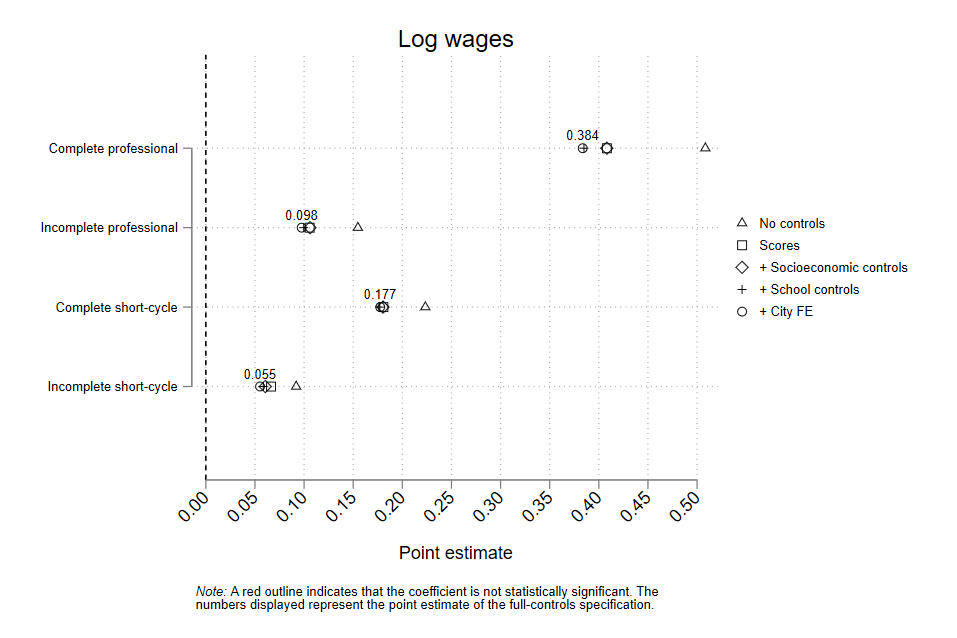
\includegraphics{Graphs/Degree type/degree_type_controls_l_salario_ultimo_obs.png}
    }
\end{frame}

\begin{frame}{Results: The role of controls}
    \centering
    \resizebox{0.7\textwidth}{!}{
      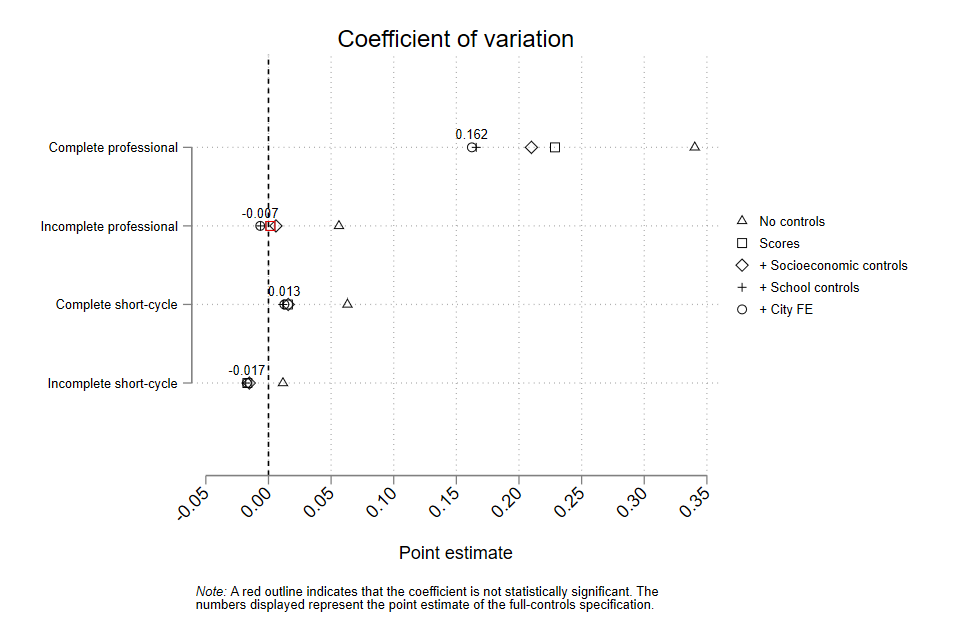
\includegraphics{Graphs/Degree type/degree_type_controls_CV.png}
    }
\end{frame}

\begin{frame}{Results: The role of controls}
    \centering
    \resizebox{0.7\textwidth}{!}{
      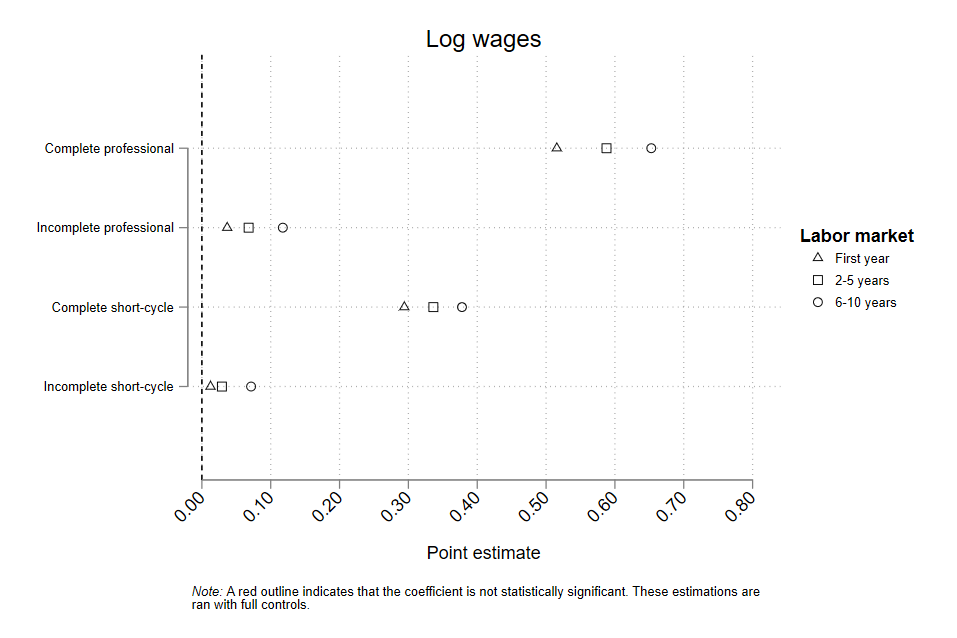
\includegraphics{Graphs/Degree type/degree_type_years_l_salario_ultimo_obs.png}
    }
\end{frame}

\begin{frame}{Results: The role of controls}
    \centering
    \resizebox{0.7\textwidth}{!}{
      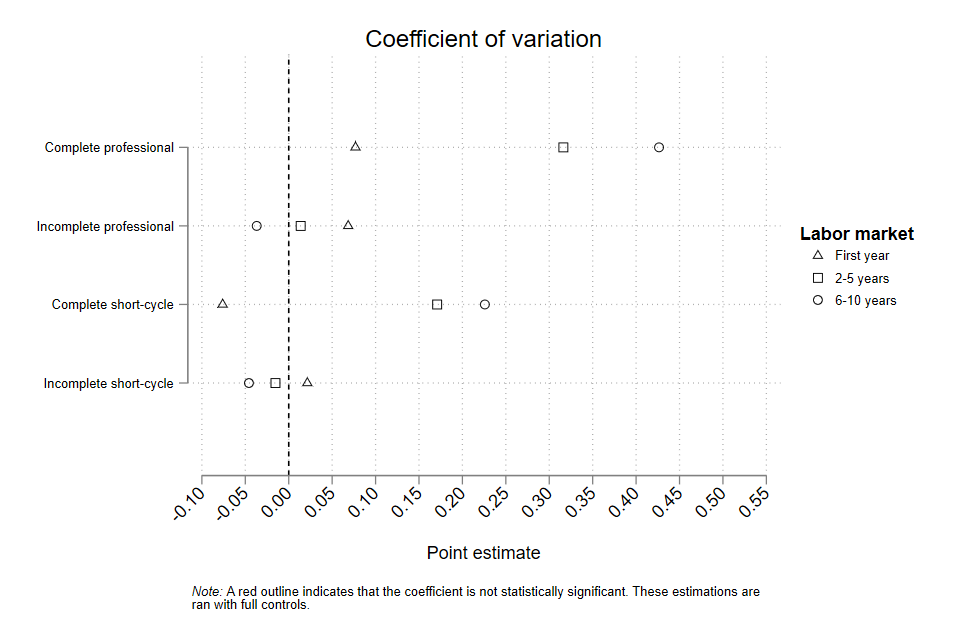
\includegraphics{Graphs/Degree type/degree_type_years_CV.png}
    }
\end{frame}

%% RIF

\begin{frame}{Results: Effects on percentiles 10, 50, and 90 (RIF)}
    \centering
    \resizebox{0.7\textwidth}{!}{
      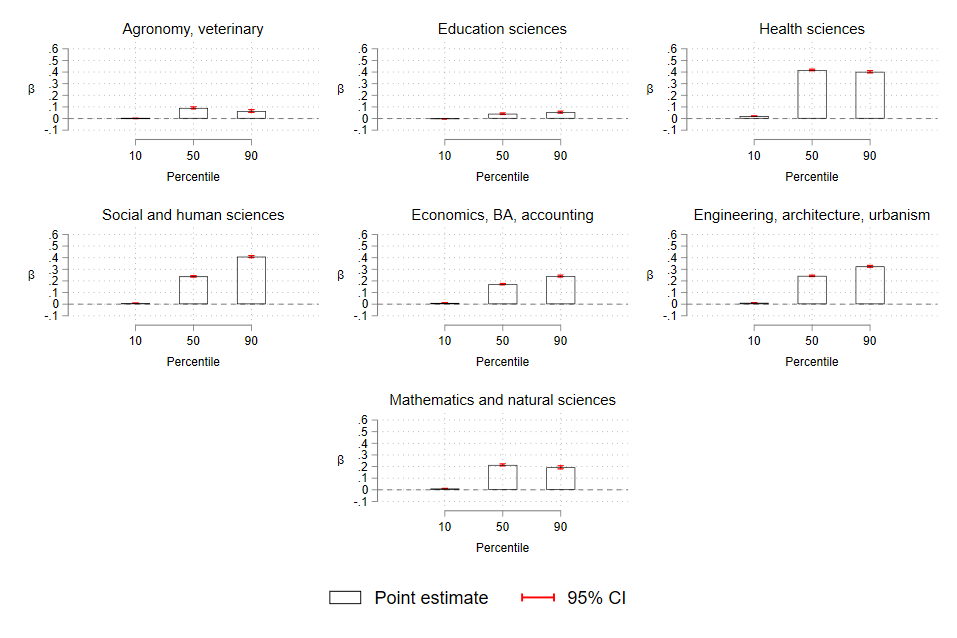
\includegraphics{Graphs/RIF/RIF_areas.png}
    }
\end{frame}

% Cities
\begin{frame}{Results: Heterogeneity in cities}
    \centering
    \resizebox{0.7\textwidth}{!}{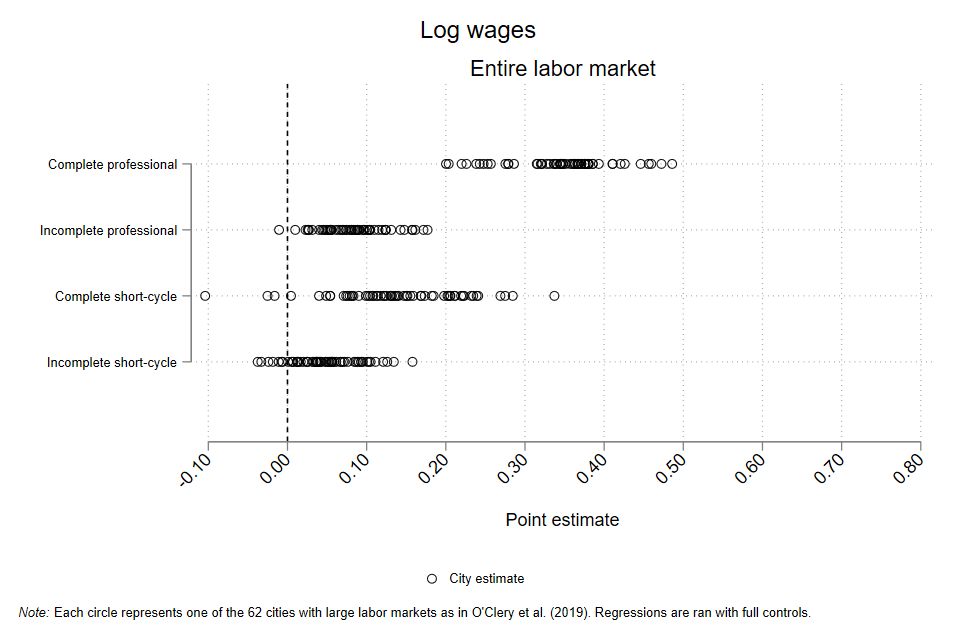
\includegraphics{Graphs/City/Degree_wages_entire_market.png}
    }
\end{frame}

\begin{frame}{Results: Heterogeneity in cities and experience}
    \centering
    \resizebox{0.7\textwidth}{!}{
    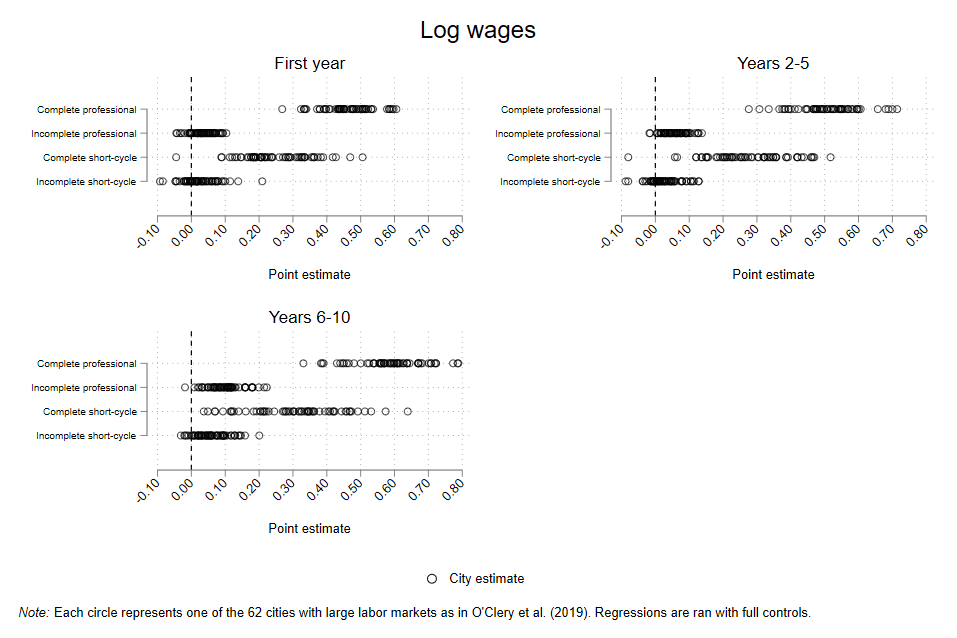
\includegraphics{Graphs/City/Degree_wages.png}
    }
\end{frame}

\begin{frame}{Results: Heterogeneity in cities (CV)}
    \centering
    \resizebox{0.7\textwidth}{!}{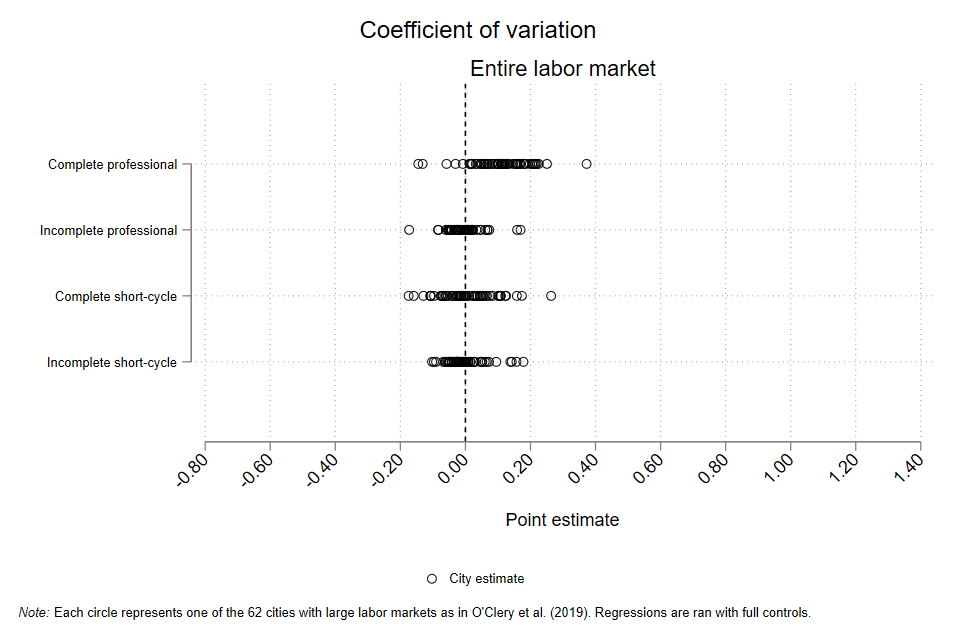
\includegraphics{Graphs/City/Degree_CV_entire_market.png}
    }
\end{frame}

\begin{frame}{Results: Heterogeneity in cities and experience (CV)}
    \centering
    \resizebox{0.7\textwidth}{!}{
    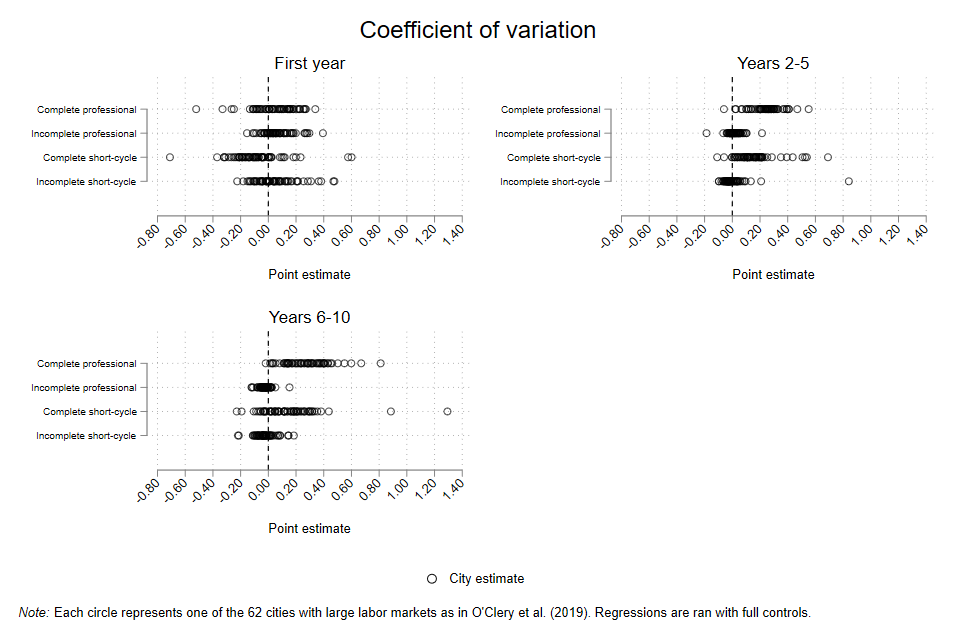
\includegraphics{Graphs/City/Degree_CV.png}
    }
\end{frame}

\begin{frame}{Estimation by field of study}
\begin{equation*}
    Y_{i t c s}=\alpha+\beta_k \mathbb{1}\left(\text {Field}_i=k\right)+X_i^{\prime} \delta+\gamma_c+\phi_s+\psi_t+\varepsilon_{i t c s}
\end{equation*}

Same as before, except:

\begin{wideitemize}
    \item The $\beta_k$ coefficients capture the effects of each type of \textit{Field of study}. These coefficients are relative to individuals whose field of study is \textbf{liberal arts}.
    \item Regressions are conditional on having accessed higher education and conditional on the four previous types of degrees within the field of study
\end{wideitemize}

\vfill
\end{frame}

\begin{frame}{Results: Field of study}
    \centering
    \resizebox{0.7\textwidth}{!}{
      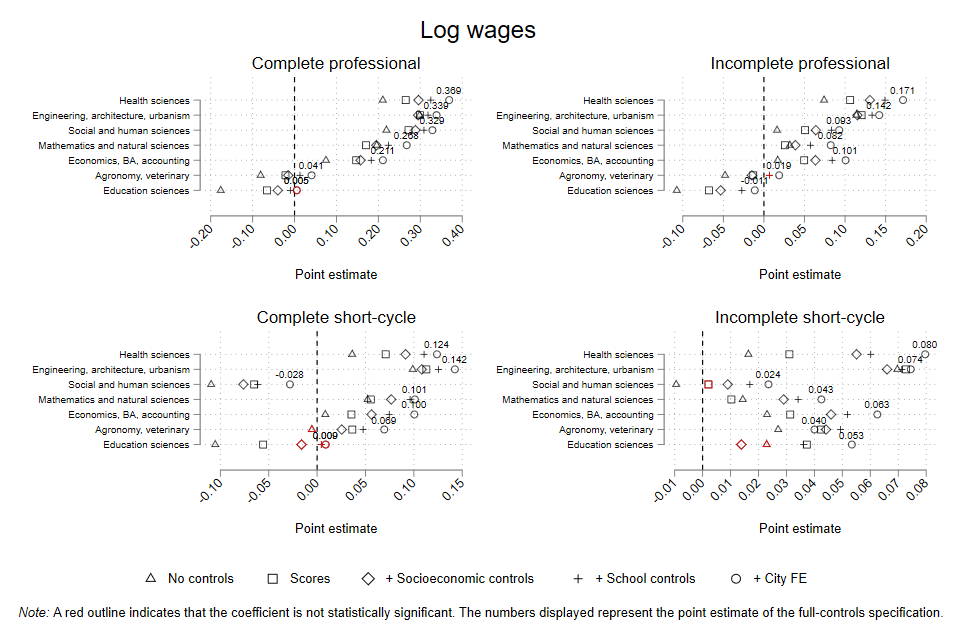
\includegraphics{Graphs/area_degree/Salario_controls.png}
    }
\end{frame}

\begin{frame}{Results: Field of study (using same x-axis)}
    \centering
    \resizebox{0.7\textwidth}{!}{
      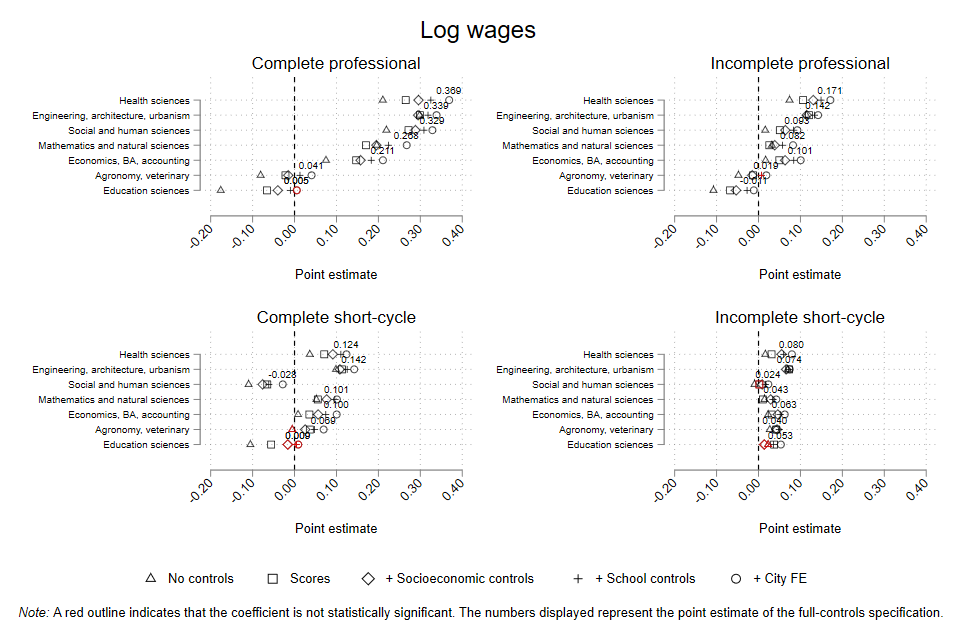
\includegraphics{Graphs/area_degree/Salario_controls_common.png}
    }
\end{frame}

\begin{frame}{Results: Field of study (CV)}
    \centering
    \resizebox{0.7\textwidth}{!}{
      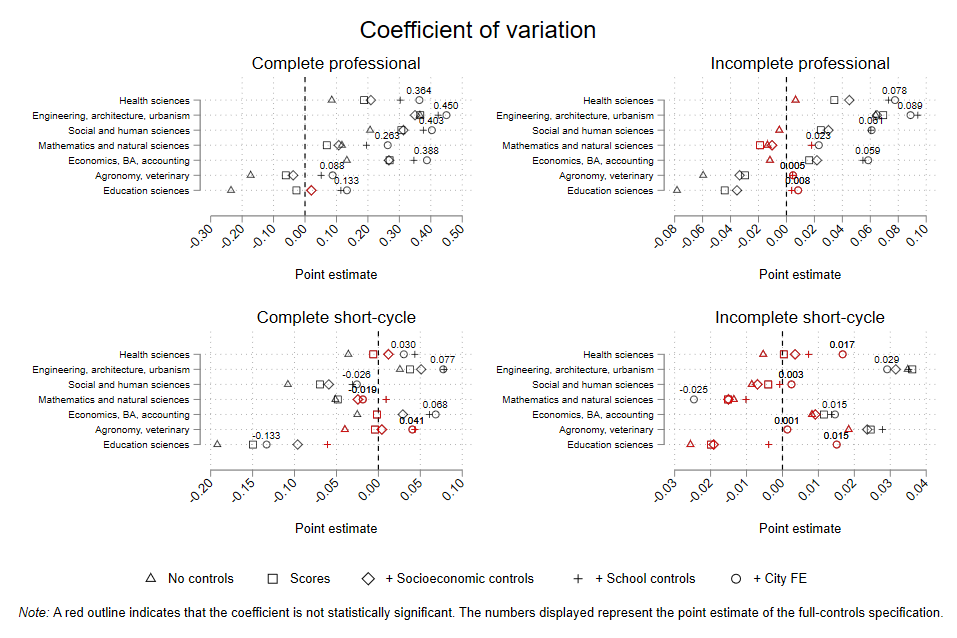
\includegraphics{Graphs/area_degree/CV_controls.png}
    }
\end{frame}

\begin{frame}{Results: Field of study (CV using same x-axis)}
    \centering
    \resizebox{0.7\textwidth}{!}{
      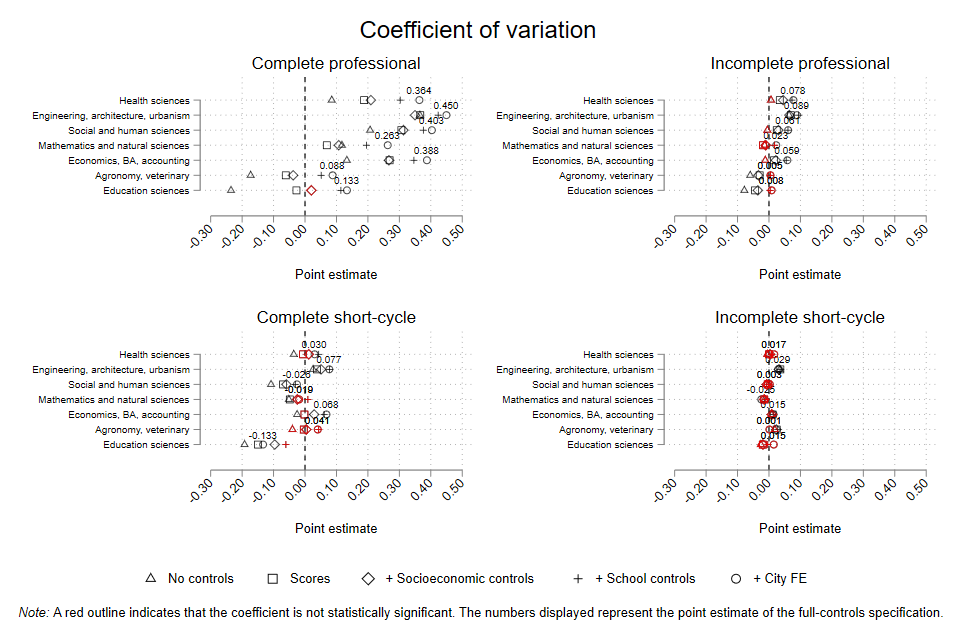
\includegraphics{Graphs/area_degree/CV_controls_common.png}
    }
\end{frame}


\begin{frame}{Results: Field of study and experience}
    \centering
    \resizebox{0.7\textwidth}{!}{
      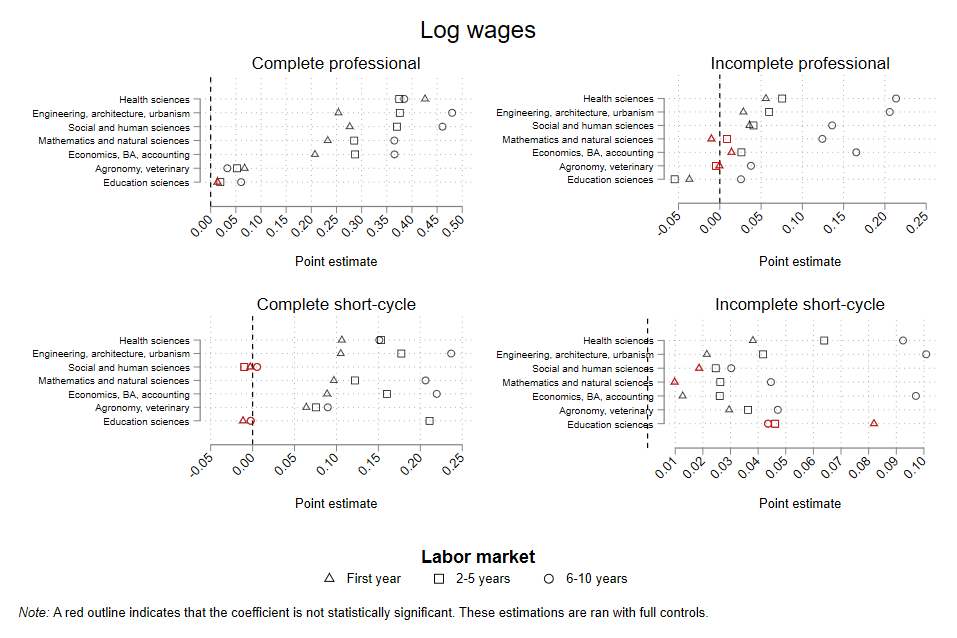
\includegraphics{Graphs/area_degree/Salario_years.png}
    }
\end{frame}

\begin{frame}{Results: Field of study and experience (using same x-axis)}
    \centering
    \resizebox{0.7\textwidth}{!}{
      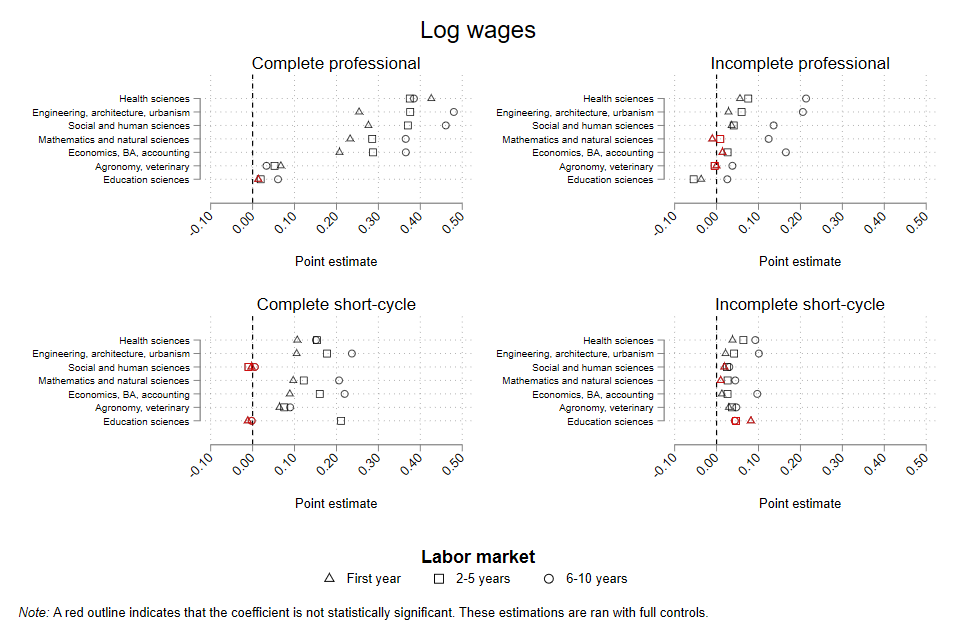
\includegraphics{Graphs/area_degree/Salario_years_common.png}
    }
\end{frame}


\begin{frame}{Results: Effects on percentiles 10, 50 and 90 (RIF) - \textbf{Complete} professional}
    \centering
    \resizebox{0.7\textwidth}{!}{
      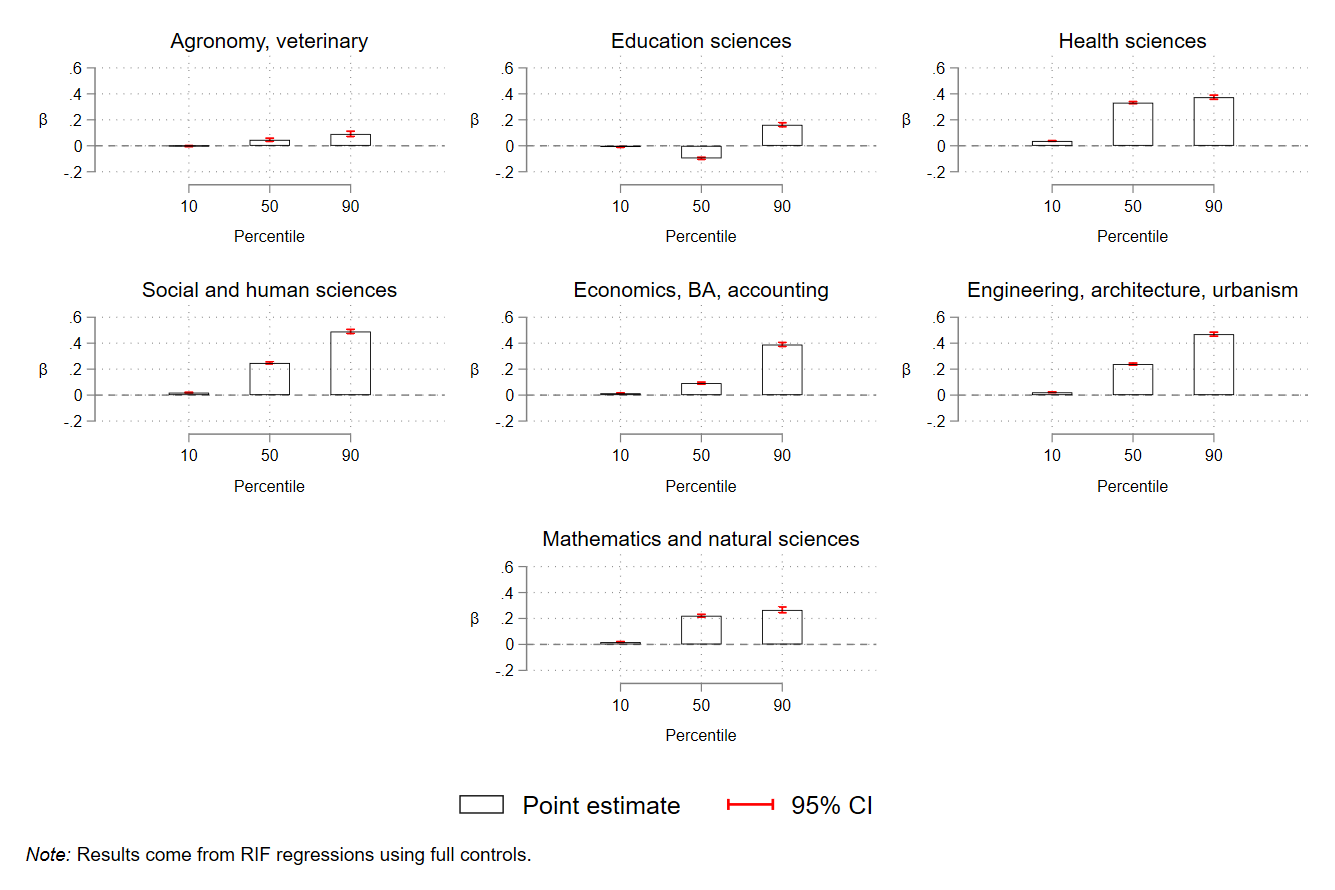
\includegraphics{Graphs/RIF/RIF_areas_grado_prof.png}
    }
\end{frame}

\begin{frame}{Results: Effects on percentiles 10, 50 and 90 (RIF) - \textbf{Incomplete} professional}
    \centering
    \resizebox{0.7\textwidth}{!}{
      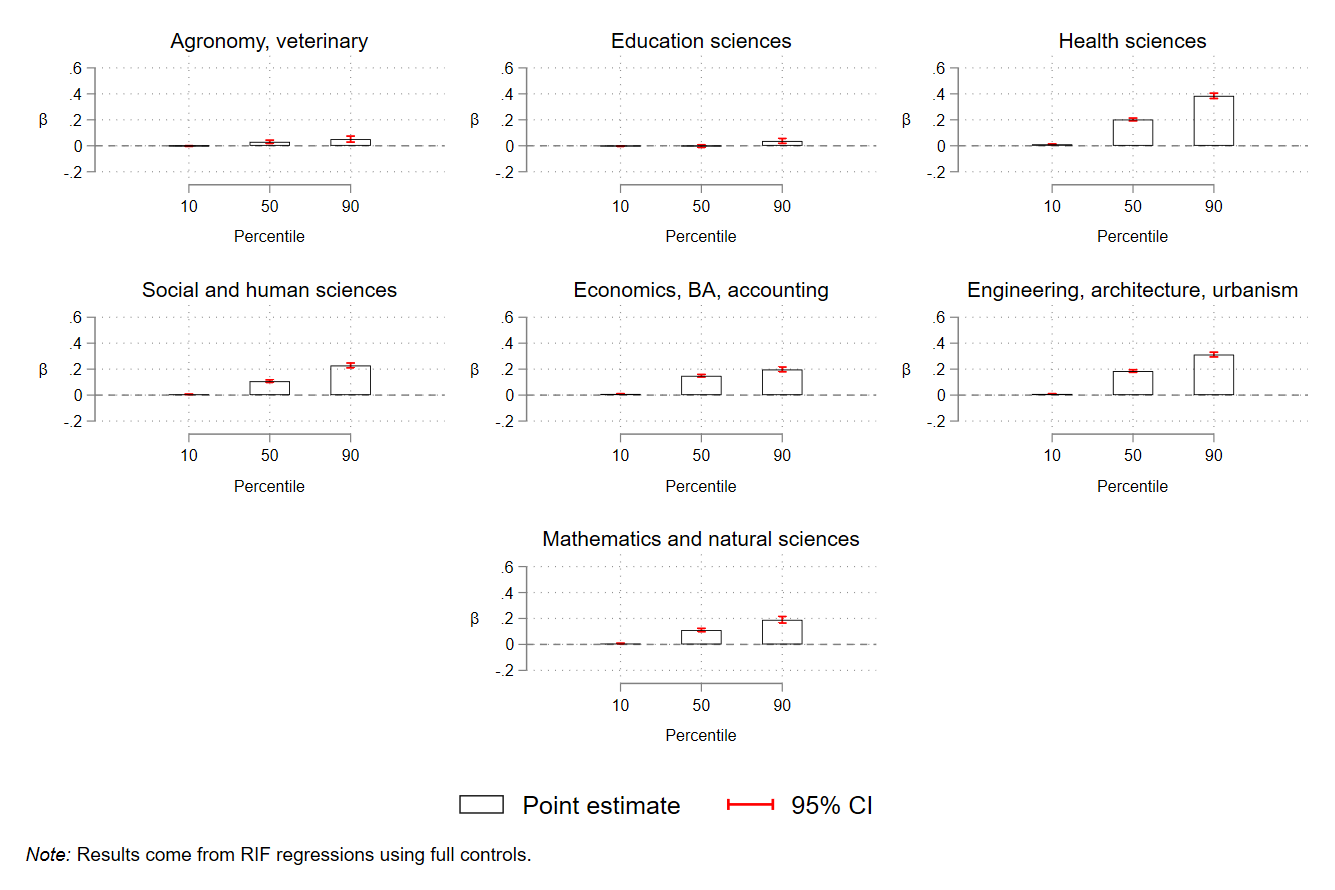
\includegraphics{Graphs/RIF/RIF_areas_incompleto_prof.png}
    }
\end{frame}


\begin{frame}{Results: Effects on percentiles 10, 50 and 90 (RIF) - \textbf{Complete} short-cycle}
    \centering
    \resizebox{0.7\textwidth}{!}{
      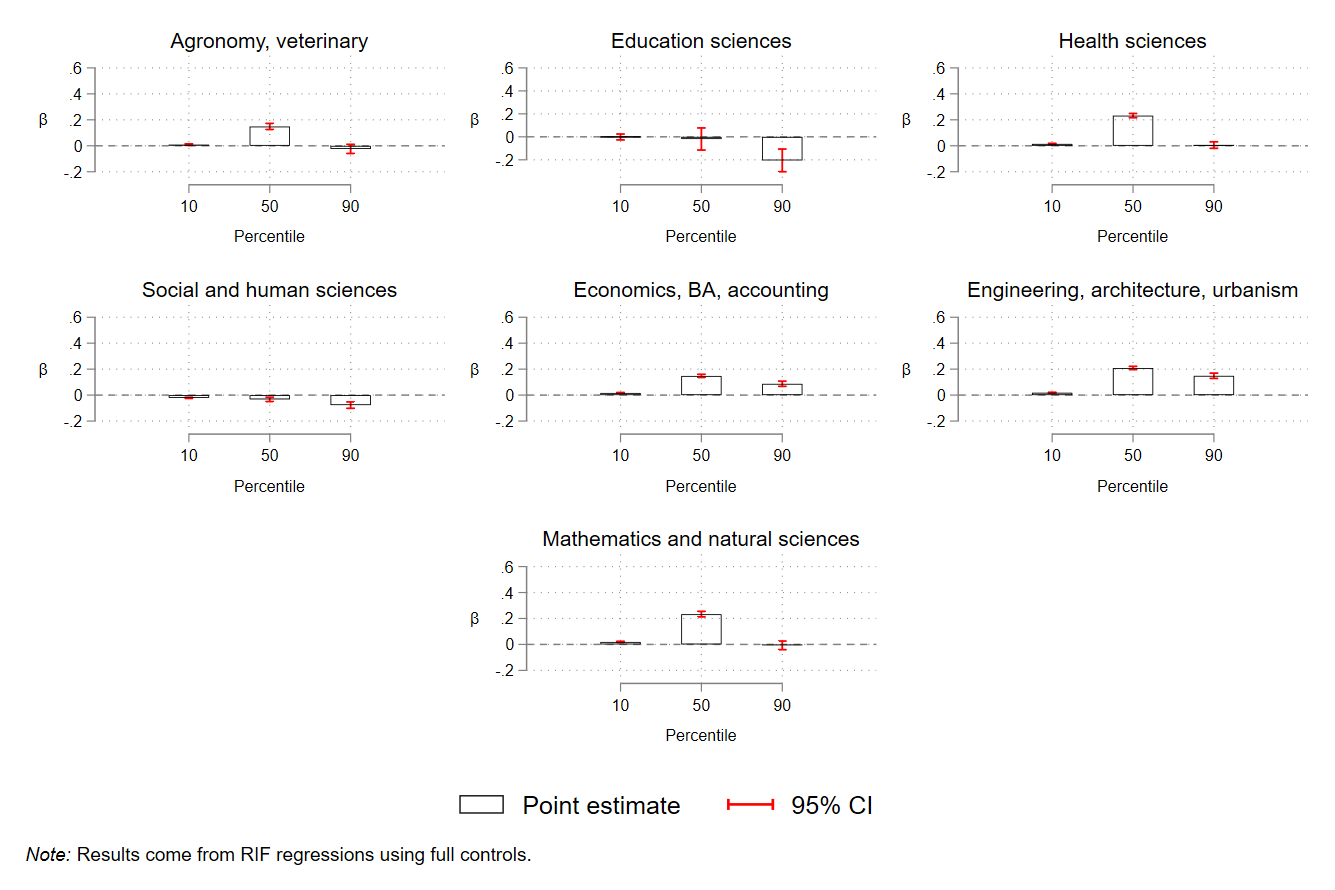
\includegraphics{Graphs/RIF/RIF_areas_grado_tyt.png}
    }
\end{frame}

\begin{frame}{Results: Effects on percentiles 10, 50 and 90 (RIF) - \textbf{Incomplete} short-cycle}
    \centering
    \resizebox{0.7\textwidth}{!}{
      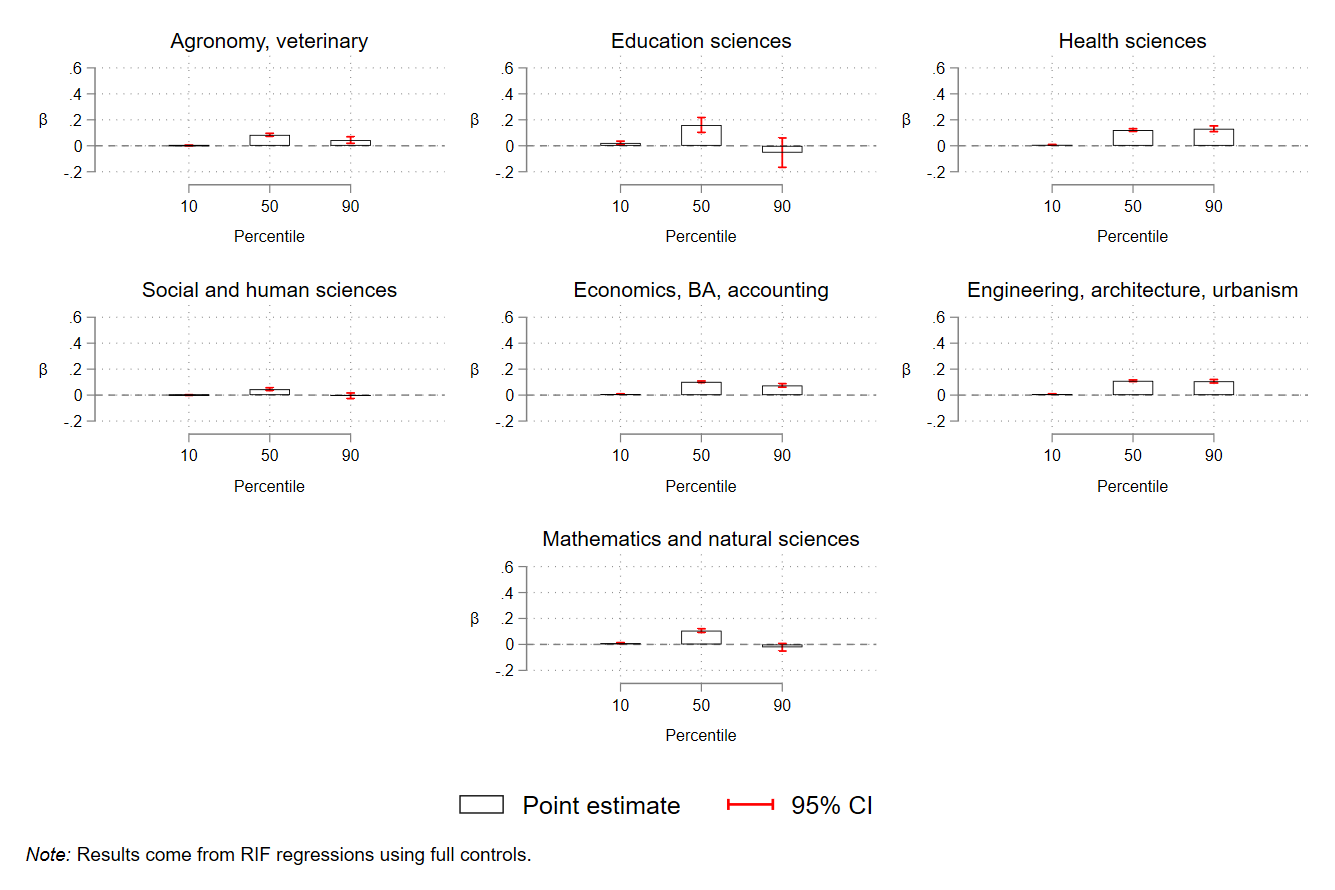
\includegraphics{Graphs/RIF/RIF_areas_incompleto_tyt.png}
    }
\end{frame}


\section*{References}
\begin{frame}[allowframebreaks]{References}
\bibliographystyle{apacite}
\tiny\bibliography{references}
\end{frame}

\end{document}


